\documentclass[11pt, a4paper]{report}

% ========== Common Packages ==========
\usepackage{fontspec}
\usepackage{kotex}
\usepackage{amsmath, amssymb, amsthm}
\usepackage{mathtools}
\usepackage{bm}
\usepackage{graphicx}
\usepackage{booktabs}
\usepackage{array}
\usepackage{tabularx}
\usepackage{longtable}
\usepackage{hyperref}
\usepackage{cleveref}
\usepackage{geometry}
\usepackage{fancyhdr}
\usepackage{titlesec}
\usepackage{enumitem}
\usepackage{xcolor}
\usepackage{tcolorbox}
\usepackage{algorithm}
\usepackage{algorithmic}
\usepackage{tikz}
\usetikzlibrary{arrows.meta, positioning, calc, decorations.pathreplacing, shapes.geometric, fit, patterns, angles, quotes, trees}
\usepackage{pgfplots}
\pgfplotsset{compat=1.18}
\usepackage{caption}
\usepackage{subcaption}
\usepackage{float}

\geometry{margin=2.5cm, top=3cm, bottom=3cm}

\usepackage{multirow}
% ========== Colors ==========
% Common
\definecolor{defblue}{RGB}{30, 80, 150}
\definecolor{thmgreen}{RGB}{20, 110, 60}
\definecolor{noteorange}{RGB}{200, 100, 0}
\definecolor{lightblue}{RGB}{230, 240, 255}
\definecolor{lightgreen}{RGB}{230, 255, 235}
\definecolor{lightorange}{RGB}{255, 245, 230}
\definecolor{lightgray}{RGB}{245, 245, 245}
% Extended
\definecolor{lightred}{RGB}{255, 235, 235}
\definecolor{darkred}{RGB}{180, 30, 30}
\definecolor{biogreen}{RGB}{10, 130, 80}
\definecolor{cvpurple}{RGB}{100, 40, 150}
\definecolor{injuryred}{RGB}{200, 40, 40}
\definecolor{codegray}{RGB}{240, 240, 245}
\definecolor{pipeblue}{RGB}{25, 100, 180}
\definecolor{constraintred}{RGB}{200, 50, 50}
\definecolor{termblack}{RGB}{30, 30, 30}
\definecolor{goldcolor}{RGB}{180, 140, 20}

% ========== tcolorbox environments ==========
% --- Common (all parts) ---
\newtcolorbox{keyidea}[1][]{
  colback=lightblue,
  colframe=defblue,
  fonttitle=\bfseries,
  title={Key Idea},
  #1
}

\newtcolorbox{importantnote}[1][]{
  colback=lightorange,
  colframe=noteorange,
  fonttitle=\bfseries,
  title={Important},
  #1
}

\newtcolorbox{summary}[1][]{
  colback=lightgreen,
  colframe=thmgreen,
  fonttitle=\bfseries,
  title={Summary},
  #1
}

% --- Warning/Error ---
\newtcolorbox{warningbox}[1][]{
  colback=lightred,
  colframe=darkred,
  fonttitle=\bfseries,
  title={Warning},
  #1
}

% --- Domain: Biomechanics & Clinical ---
\newtcolorbox{clinicalnote}[1][]{
  colback=lightred,
  colframe=darkred,
  fonttitle=\bfseries,
  title={Clinical Note},
  #1
}

\newtcolorbox{biomechbox}[1][]{
  colback=lightgreen,
  colframe=biogreen,
  fonttitle=\bfseries,
  title={Biomechanics},
  #1
}

\newtcolorbox{injurybox}[1][]{
  colback={injuryred!8},
  colframe=injuryred,
  fonttitle=\bfseries,
  title={Injury Risk},
  #1
}

% --- Domain: Computer Vision ---
\newtcolorbox{cvbox}[1][]{
  colback={cvpurple!5},
  colframe=cvpurple,
  fonttitle=\bfseries,
  title={Computer Vision},
  #1
}

% --- Pipeline & Setup ---
\newtcolorbox{setupbox}[1][]{
  colback=lightgray,
  colframe=gray!60,
  fonttitle=\bfseries,
  title={Setup},
  #1
}

\newtcolorbox{pipelinebox}[1][]{
  colback=pipeblue!5,
  colframe=pipeblue,
  fonttitle=\bfseries,
  title={Pipeline Step},
  #1
}

\newtcolorbox{codebox}[1][]{
  colback=codegray,
  colframe=gray!70,
  fonttitle=\bfseries\ttfamily,
  title={Code},
  #1
}

\newtcolorbox{termbox}[1][]{
  colback=termblack!5,
  colframe=termblack!60,
  fonttitle=\bfseries\ttfamily,
  title={Terminal},
  #1
}

% --- Research ---
\newtcolorbox{hypothesis}[1][]{
  colback=goldcolor!8,
  colframe=goldcolor,
  fonttitle=\bfseries,
  title={Hypothesis},
  #1
}

\newtcolorbox{resultbox}[1][]{
  colback=thmgreen!8,
  colframe=thmgreen,
  fonttitle=\bfseries,
  title={Expected Result},
  #1
}

% --- Constraints & Solutions ---
\newtcolorbox{constraintbox}[1][]{
  colback=constraintred!8,
  colframe=constraintred,
  fonttitle=\bfseries,
  title={Constraint},
  #1
}

\newtcolorbox{solutionbox}[1][]{
  colback=thmgreen!8,
  colframe=thmgreen,
  fonttitle=\bfseries,
  title={Solution},
  #1
}

\newtcolorbox{databox}[1][]{
  colback=pipeblue!5,
  colframe=pipeblue,
  fonttitle=\bfseries,
  title={Data Spec},
  #1
}

% --- Progress/Status ---
\newtcolorbox{successbox}[1][]{
  colback=lightgreen,
  colframe=thmgreen,
  fonttitle=\bfseries,
  title={Success},
  #1
}

\newtcolorbox{nextbox}[1][]{
  colback=lightorange,
  colframe=noteorange,
  fonttitle=\bfseries,
  title={Next Step},
  #1
}

% --- Fitting guide ---
\newtcolorbox{failbox}[1][]{
  colback=lightred,
  colframe=darkred,
  fonttitle=\bfseries,
  title={Failure Pattern},
  #1
}

\newtcolorbox{fixbox}[1][]{
  colback=lightgreen,
  colframe=thmgreen,
  fonttitle=\bfseries,
  title={Fix},
  #1
}

\newtcolorbox{lessonbox}[1][]{
  colback=lightorange,
  colframe=noteorange,
  fonttitle=\bfseries,
  title={Lesson Learned},
  #1
}

% --- Specification ---
\newtcolorbox{specbox}[1][]{
  colback=cvpurple!5,
  colframe=cvpurple,
  fonttitle=\bfseries,
  title={Specification},
  #1
}

\newtcolorbox{checklistbox}[1][]{
  colback=lightgreen,
  colframe=biogreen,
  fonttitle=\bfseries,
  title={Checklist},
  #1
}

% ========== Custom math commands ==========
% Vectors (lowercase)
\newcommand{\vx}{\mathbf{x}}
\newcommand{\vd}{\mathbf{d}}
\newcommand{\vo}{\mathbf{o}}
\newcommand{\vc}{\mathbf{c}}
\newcommand{\vr}{\mathbf{r}}
\newcommand{\vp}{\mathbf{p}}
\newcommand{\vv}{\mathbf{v}}
\newcommand{\vn}{\mathbf{n}}
\newcommand{\vu}{\mathbf{u}}
\newcommand{\vt}{\mathbf{t}}
\newcommand{\ve}{\mathbf{e}}
\newcommand{\vq}{\mathbf{q}}
% Vectors (uppercase)
\newcommand{\vF}{\mathbf{F}}
\newcommand{\vM}{\mathbf{M}}
\newcommand{\va}{\mathbf{a}}
\newcommand{\vg}{\mathbf{g}}
\newcommand{\vX}{\mathbf{X}}
% Bold Greek
\newcommand{\vmu}{\bm{\mu}}
\newcommand{\vbeta}{\bm{\beta}}
\newcommand{\vtheta}{\bm{\theta}}
\newcommand{\vpsi}{\bm{\psi}}
% Matrices
\newcommand{\mSigma}{\bm{\Sigma}}
\newcommand{\mR}{\mathbf{R}}
\newcommand{\mS}{\mathbf{S}}
\newcommand{\mW}{\mathbf{W}}
\newcommand{\mJ}{\mathbf{J}}
\newcommand{\mG}{\mathbf{G}}
\newcommand{\mT}{\mathbf{T}}
\newcommand{\mI}{\mathbf{I}}
\newcommand{\mB}{\mathbf{B}}
\newcommand{\mK}{\mathbf{K}}
\newcommand{\mP}{\mathbf{P}}
\newcommand{\mF}{\mathbf{F}}
\newcommand{\mE}{\mathbf{E}}
\newcommand{\mA}{\mathbf{A}}
\newcommand{\mH}{\mathbf{H}}
% Sets and groups
\newcommand{\RR}{\mathbb{R}}
\newcommand{\SO}{\mathrm{SO}}
% Units
\newcommand{\degps}{\,\text{deg/s}}
\newcommand{\Nm}{\ensuremath{\,\text{N}\cdot\text{m}}}
\newcommand{\BW}{\,\text{BW}}

% ========== Listings ==========
\usepackage{listings}

\lstset{
  basicstyle=\ttfamily\small,
  keywordstyle=\color{defblue}\bfseries,
  commentstyle=\color{thmgreen}\itshape,
  stringstyle=\color{noteorange},
  backgroundcolor=\color{codegray},
  frame=single,
  rulecolor=\color{gray!40},
  breaklines=true,
  showstringspaces=false,
  numbers=left,
  numberstyle=\tiny\color{gray},
  tabsize=4,
  captionpos=b
}

% ========== Header/Footer ==========
\pagestyle{fancy}
\fancyhf{}
\fancyhead[L]{\leftmark}
\fancyhead[R]{\thepage}
\renewcommand{\headrulewidth}{0.4pt}

% ========== Title formatting ==========
\titleformat{\chapter}[display]
  {\normalfont\huge\bfseries\color{defblue}}
  {\chaptertitlename\ \thechapter}{20pt}{\Huge}

\titleformat{\section}
  {\normalfont\Large\bfseries\color{defblue!80!black}}
  {\thesection}{1em}{}

\titleformat{\subsection}
  {\normalfont\large\bfseries\color{defblue!60!black}}
  {\thesubsection}{1em}{}


\begin{document}

% ==================== TITLE PAGE ====================
\begin{titlepage}
\centering
\vspace*{1.5cm}
{\Large\color{gray} GART-Pitch Development Guide}
\vspace{0.5cm}

{\Huge\bfseries\color{defblue} GART-Pitch\\[0.3cm]
개발 환경 세팅 가이드}

\vspace{0.8cm}

{\LARGE\color{defblue!70!black} 하드웨어, 소프트웨어, 데이터 파이프라인\\
A-to-Z 실전 구축 매뉴얼}

\vspace{1.5cm}

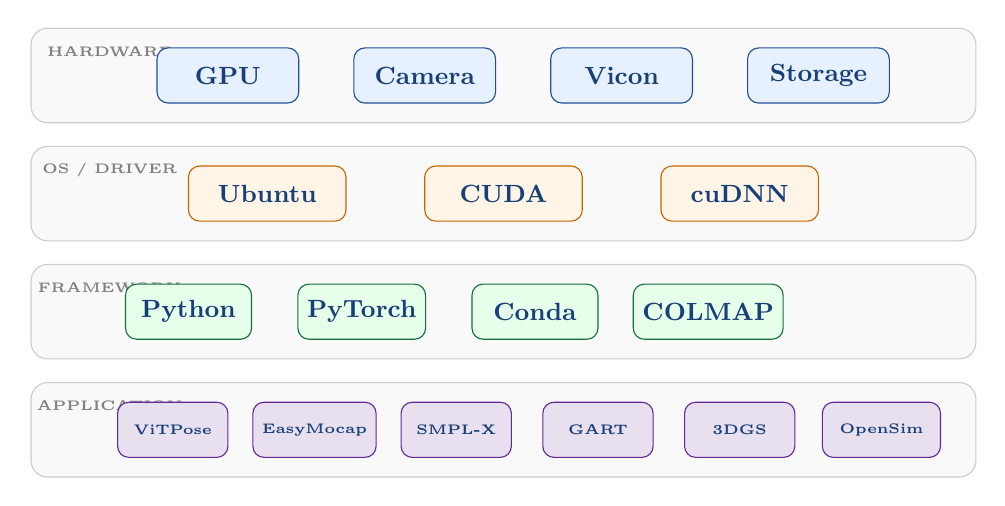
\begin{tikzpicture}[
  block/.style={rectangle, rounded corners=4pt, draw=defblue, fill=lightblue,
    minimum width=2.2cm, minimum height=0.7cm, font=\small\bfseries, text=defblue!80!black, align=center},
  arrow/.style={-Stealth, thick, defblue!60},
  layer/.style={rectangle, rounded corners=6pt, draw=gray!40, fill=gray!5, minimum width=12cm}
]
% Hardware layer
\node[layer, minimum height=1.2cm] (hw) at (0, 3) {};
\node[font=\tiny\bfseries\color{gray}] at (-5, 3.3) {HARDWARE};
\node[block, minimum width=1.8cm] at (-3.5, 3) {GPU};
\node[block, minimum width=1.8cm] at (-1, 3) {Camera};
\node[block, minimum width=1.8cm] at (1.5, 3) {Vicon};
\node[block, minimum width=1.8cm] at (4, 3) {Storage};

% OS layer
\node[layer, minimum height=1.2cm] (os) at (0, 1.5) {};
\node[font=\tiny\bfseries\color{gray}] at (-5, 1.8) {OS / DRIVER};
\node[block, fill=lightorange, draw=noteorange, minimum width=2cm] at (-3, 1.5) {Ubuntu};
\node[block, fill=lightorange, draw=noteorange, minimum width=2cm] at (0, 1.5) {CUDA};
\node[block, fill=lightorange, draw=noteorange, minimum width=2cm] at (3, 1.5) {cuDNN};

% Framework layer
\node[layer, minimum height=1.2cm] (fw) at (0, 0) {};
\node[font=\tiny\bfseries\color{gray}] at (-5, 0.3) {FRAMEWORK};
\node[block, fill=lightgreen, draw=thmgreen, minimum width=1.6cm] at (-4, 0) {Python};
\node[block, fill=lightgreen, draw=thmgreen, minimum width=1.6cm] at (-1.8, 0) {PyTorch};
\node[block, fill=lightgreen, draw=thmgreen, minimum width=1.6cm] at (0.4, 0) {Conda};
\node[block, fill=lightgreen, draw=thmgreen, minimum width=1.6cm] at (2.6, 0) {COLMAP};

% App layer
\node[layer, minimum height=1.2cm] (app) at (0, -1.5) {};
\node[font=\tiny\bfseries\color{gray}] at (-5, -1.2) {APPLICATION};
\node[block, fill=cvpurple!15, draw=cvpurple, minimum width=1.4cm, font=\tiny\bfseries] at (-4.2, -1.5) {ViTPose};
\node[block, fill=cvpurple!15, draw=cvpurple, minimum width=1.5cm, font=\tiny\bfseries] at (-2.4, -1.5) {EasyMocap};
\node[block, fill=cvpurple!15, draw=cvpurple, minimum width=1.4cm, font=\tiny\bfseries] at (-0.6, -1.5) {SMPL-X};
\node[block, fill=cvpurple!15, draw=cvpurple, minimum width=1.4cm, font=\tiny\bfseries] at (1.2, -1.5) {GART};
\node[block, fill=cvpurple!15, draw=cvpurple, minimum width=1.4cm, font=\tiny\bfseries] at (3, -1.5) {3DGS};
\node[block, fill=cvpurple!15, draw=cvpurple, minimum width=1.5cm, font=\tiny\bfseries] at (4.8, -1.5) {OpenSim};
\end{tikzpicture}

\vspace{1.5cm}
{\large 2026}

\vspace{\fill}
{\small\color{gray} Part 5 연구 제안서(GART-Pitch) 구현을 위한\\
하드웨어$\cdot$소프트웨어$\cdot$데이터 환경 구축 실전 가이드.}
\end{titlepage}

\tableofcontents
\newpage


% ====================================================================
% CHAPTER 1: 전체 아키텍처 개요
% ====================================================================
\chapter{전체 아키텍처 개요}
\label{ch:overview}

\section{GART-Pitch 파이프라인 구성요소}

\begin{figure}[H]
\centering
\begin{tikzpicture}[
  block/.style={rectangle, rounded corners=3pt, draw, minimum width=2.5cm, minimum height=0.7cm,
    align=center, font=\small},
  arrow/.style={-{Stealth[length=2mm]}, thick},
  node distance=0.5cm
]
% Stage 0: Data
\node[block, fill=lightorange, draw=noteorange] (data) at (0,0) {0. 데이터 수집\\7$\times$240Hz + Vicon};

% Stage 1: Preprocessing
\node[block, fill=lightgray, draw=gray] (sync) at (0,-1.5) {1a. 동기화\\ffmpeg + 크로스상관};
\node[block, fill=lightgray, draw=gray] (calib) at (5,-1.5) {1b. 카메라 보정\\COLMAP};

% Stage 2: 2D Pose
\node[block, fill=lightblue, draw=defblue] (pose2d) at (0,-3) {2. 2D 자세 추정\\ViTPose / MMPose};

% Stage 3: SMPL-X
\node[block, fill=cvpurple!15, draw=cvpurple] (smpl) at (0,-4.5) {3. SMPL-X 피팅\\EasyMocap};

% Stage 4: GART
\node[block, fill=defblue!20, draw=defblue] (gart) at (0,-6) {4. GART 학습\\+ 자세 정제};

% Stage 5: Biomech
\node[block, fill=lightgreen, draw=biogreen] (bio) at (0,-7.5) {5. 생체역학\\OpenSim IK/ID};

% Stage 6: Validation
\node[block, fill=thmgreen!20, draw=thmgreen] (val) at (0,-9) {6. Vicon 검증\\Bland-Altman, ICC};

% Arrows
\draw[arrow] (data) -- (sync);
\draw[arrow] (data) -| (calib);
\draw[arrow] (sync) -- (pose2d);
\draw[arrow] (calib) -- ++(0,-1) -| (pose2d);
\draw[arrow] (pose2d) -- (smpl);
\draw[arrow] (smpl) -- (gart);
\draw[arrow] (gart) -- (bio);
\draw[arrow] (bio) -- (val);

% Tools on the right
\node[font=\scriptsize\color{gray}, right=0.5cm] at (sync.east) {ffmpeg, numpy, scipy};
\node[font=\scriptsize\color{gray}, right=0.5cm] at (calib.east) {COLMAP, OpenCV};
\node[font=\scriptsize\color{gray}, right=0.5cm] at (pose2d.east) {MMPose, ViTPose, PyTorch};
\node[font=\scriptsize\color{gray}, right=0.5cm] at (smpl.east) {smplx, EasyMocap, PyTorch};
\node[font=\scriptsize\color{gray}, right=0.5cm] at (gart.east) {gaussian-splatting, diff-rasterizer};
\node[font=\scriptsize\color{gray}, right=0.5cm] at (bio.east) {opensim-python, scipy};
\node[font=\scriptsize\color{gray}, right=0.5cm] at (val.east) {pingouin, matplotlib};

\end{tikzpicture}
\caption{GART-Pitch 개발 파이프라인과 각 단계별 핵심 도구}
\end{figure}

\begin{keyidea}
전체 파이프라인은 7개 단계, 약 15개의 핵심 소프트웨어 컴포넌트로 구성된다.
각 단계는 독립적으로 테스트 가능하며, 순차적으로 구축하는 것을 권장한다.
가장 까다로운 설치는 \textbf{Stage 4 (GART/3DGS)}의 CUDA 커스텀 래스터라이저이다.
\end{keyidea}


% ====================================================================
% CHAPTER 2: 하드웨어 요구사항
% ====================================================================
\chapter{하드웨어 요구사항}
\label{ch:hardware}

\section{컴퓨팅 하드웨어}

\begin{table}[H]
\centering
\caption{컴퓨팅 하드웨어 사양 (최소 / 권장 / 최적)}
\label{tab:compute_hw}
\renewcommand{\arraystretch}{1.3}
\begin{tabularx}{\textwidth}{lXXX}
\toprule
\textbf{항목} & \textbf{최소} & \textbf{권장} & \textbf{최적} \\
\midrule
\textbf{GPU} & RTX 3090 (24GB) & RTX 4090 (24GB) & A100 80GB / H100 \\
\textbf{GPU VRAM} & 24 GB & 24 GB & 48--80 GB \\
\textbf{CPU} & 8코어 & 16코어+ (i9/Ryzen 9) & 32코어+ (Threadripper) \\
\textbf{RAM} & 32 GB & 64 GB & 128 GB \\
\textbf{스토리지} & 1 TB NVMe SSD & 2 TB NVMe SSD & 4 TB+ NVMe SSD \\
\textbf{OS} & Ubuntu 22.04 LTS & Ubuntu 22.04 LTS & Ubuntu 22.04/24.04 \\
\bottomrule
\end{tabularx}
\end{table}

\begin{warningbox}
\textbf{GPU VRAM이 가장 중요한 병목이다.}
GART는 프레임당 100K--500K Gaussian을 처리하며,
7대 카메라 1080p 렌더링 시 피크 VRAM $\sim$18--22 GB가 필요하다.
24GB 미만에서는 배치 크기 축소 또는 해상도 다운샘플링이 필요하다.
\end{warningbox}


\section{촬영 하드웨어}

\begin{table}[H]
\centering
\caption{촬영 장비 사양}
\label{tab:capture_hw}
\renewcommand{\arraystretch}{1.3}
\begin{tabularx}{\textwidth}{lX}
\toprule
\textbf{장비} & \textbf{사양} \\
\midrule
\textbf{RGB 카메라 $\times$7} &
  240 Hz 이상, 1920$\times$1080.
  권장: GoPro Hero 12 (240fps), Sony RX0 II, 또는 산업용 카메라 (FLIR Blackfly S).
  노출시간: $\leq$ 1/1000초 (모션블러 방지). \\
\addlinespace
\textbf{Vicon 시스템} &
  12대+ 적외선 카메라, 250--500 Hz.
  Vicon Vantage/Vero 또는 동급.
  반사 마커 39--59개 (상지 강화 마커세트). \\
\addlinespace
\textbf{동기화 장치} &
  Vicon Lock (하드웨어 genlock) 또는 오디오 기반 소프트웨어 동기화.
  시간 정밀도: $< 1$\,ms 필요. \\
\addlinespace
\textbf{보정 도구} &
  ChArUco 보드 (A2 이상). Vicon 마커 + 체커보드 코너 겸용.
  정적 보정용 + 동적 보정용 각 1매. \\
\addlinespace
\textbf{조명} &
  1000+ lux 균일 조명 (LED 패널 권장).
  고속 촬영에서 짧은 노출 보상 필수. 형광등 플리커 주의 (50/60Hz). \\
\addlinespace
\textbf{저장 장치} &
  촬영용: 카메라별 V30+ microSD 256GB 이상.
  아카이브: 10명 연구 기준 ProRes $\sim$3 TB, H.265 $\sim$90 GB. \\
\bottomrule
\end{tabularx}
\end{table}

\section{데이터 저장량 산정}

\begin{table}[H]
\centering
\caption{포맷별 데이터 저장량 (7대 카메라 기준)}
\label{tab:storage}
\renewcommand{\arraystretch}{1.3}
\begin{tabular}{lcccl}
\toprule
\textbf{포맷} & \textbf{투구 1회 (2초)} & \textbf{세션 (100투)} & \textbf{10명 연구} & \textbf{품질} \\
\midrule
RAW & $\sim$20 GB & $\sim$2 TB & $\sim$20 TB & 무손실 \\
ProRes 422 HQ & 2--3 GB & 200--300 GB & 2--3 TB & 거의 무손실 \\
H.264 (고품질) & 100--175 MB & 10--17.5 GB & 100--175 GB & 약간의 손실 \\
H.265 (고품질) & 50--90 MB & 5--9 GB & 50--90 GB & 약간의 손실 \\
\bottomrule
\end{tabular}
\end{table}

\begin{importantnote}
3DGS 학습에서는 \textbf{광도 손실(photometric loss)}이 목적함수이므로
압축 아티팩트가 노이즈로 작용한다.
\textbf{분석용 아카이브는 ProRes 이상}, 3DGS 학습용은 \textbf{고품질 H.265}가 실용적 절충안이다.
\end{importantnote}


% ====================================================================
% CHAPTER 3: 소프트웨어 환경 구축
% ====================================================================
\chapter{소프트웨어 환경 구축}
\label{ch:software}

\section{운영체제 및 드라이버}

\begin{table}[H]
\centering
\caption{기본 시스템 요구사항}
\label{tab:system_req}
\renewcommand{\arraystretch}{1.3}
\begin{tabular}{lll}
\toprule
\textbf{항목} & \textbf{버전} & \textbf{비고} \\
\midrule
OS & Ubuntu 22.04 LTS & 24.04도 호환; macOS는 전처리만 가능 \\
NVIDIA Driver & $\geq$ 535 & \texttt{nvidia-smi}로 확인 \\
CUDA Toolkit & 11.8 또는 12.1 & PyTorch 빌드 버전과 일치 필수 \\
cuDNN & $\geq$ 8.9 & CUDA 버전에 맞는 것 \\
GCC / G++ & 11.x & CUDA 커스텀 커널 빌드에 필요 \\
\bottomrule
\end{tabular}
\end{table}

\begin{termbox}[title={NVIDIA 드라이버 + CUDA 설치}]
\begin{lstlisting}[language=bash, numbers=none]
# 1. NVIDIA 드라이버 (최신 안정 버전)
sudo apt update && sudo apt install -y nvidia-driver-535
sudo reboot

# 2. CUDA 11.8 (runfile 방식 - 가장 확실)
wget https://developer.download.nvidia.com/compute/cuda/11.8.0/
  local_installers/cuda_11.8.0_520.61.05_linux.run
sudo sh cuda_11.8.0_520.61.05_linux.run --toolkit --silent

# 3. 환경변수 설정 (~/.bashrc)
export CUDA_HOME=/usr/local/cuda-11.8
export PATH=$CUDA_HOME/bin:$PATH
export LD_LIBRARY_PATH=$CUDA_HOME/lib64:$LD_LIBRARY_PATH

# 4. 확인
nvidia-smi          # 드라이버 및 GPU 확인
nvcc --version      # CUDA 버전 확인
\end{lstlisting}
\end{termbox}


\section{Python 환경 (Conda)}

\begin{termbox}[title={Conda 환경 생성}]
\begin{lstlisting}[language=bash, numbers=none]
# Miniconda 설치 (이미 설치되어 있으면 생략)
wget https://repo.anaconda.com/miniconda/
  Miniconda3-latest-Linux-x86_64.sh
bash Miniconda3-latest-Linux-x86_64.sh -b -p ~/miniconda3
eval "$(~/miniconda3/bin/conda shell.bash hook)"

# GART-Pitch 전용 환경 생성
conda create -n gart-pitch python=3.10 -y
conda activate gart-pitch

# PyTorch (CUDA 11.8 빌드)
pip install torch==2.1.0 torchvision==0.16.0 \
    --index-url https://download.pytorch.org/whl/cu118

# GPU 확인
python -c "import torch; print(torch.cuda.is_available())"
python -c "import torch; print(torch.cuda.get_device_name(0))"
\end{lstlisting}
\end{termbox}

\begin{warningbox}
\textbf{PyTorch와 CUDA 버전 불일치가 가장 흔한 설치 실패 원인이다.}
\texttt{nvcc --version}의 CUDA와 \texttt{torch.version.cuda}가 반드시 일치해야 한다.
CUDA 12.1을 사용할 경우 \texttt{cu121} 빌드를 설치한다.
\end{warningbox}


\section{핵심 Python 패키지}

\begin{table}[H]
\centering
\caption{핵심 Python 의존성}
\label{tab:python_deps}
\renewcommand{\arraystretch}{1.2}
\small
\begin{tabular}{llll}
\toprule
\textbf{패키지} & \textbf{버전} & \textbf{용도} & \textbf{설치} \\
\midrule
\multicolumn{4}{l}{\textbf{--- 기본 과학 계산 ---}} \\
numpy & $\geq$1.24 & 수치 연산 & pip \\
scipy & $\geq$1.11 & 신호처리, 최적화, 회전 & pip \\
opencv-python & $\geq$4.8 & 영상처리, 보정 & pip \\
matplotlib & $\geq$3.7 & 시각화 & pip \\
\midrule
\multicolumn{4}{l}{\textbf{--- 3D 모델링 ---}} \\
smplx & 0.1.28+ & SMPL-X 인체 모델 & pip \\
trimesh & $\geq$3.23 & 3D 메시 처리 & pip \\
pyrender & 0.1.45+ & 3D 렌더링 시각화 & pip \\
open3d & $\geq$0.17 & 점군 시각화/처리 & pip \\
\midrule
\multicolumn{4}{l}{\textbf{--- 생체역학 ---}} \\
opensim & 4.5+ & 역운동학/역동역학 & conda-forge \\
pingouin & $\geq$0.5.3 & ICC, Bland-Altman & pip \\
\midrule
\multicolumn{4}{l}{\textbf{--- 기타 ---}} \\
tqdm & --- & 진행률 표시 & pip \\
tensorboard & --- & 학습 모니터링 & pip \\
wandb & --- & 실험 관리 (선택) & pip \\
\bottomrule
\end{tabular}
\end{table}

\begin{termbox}[title={기본 패키지 일괄 설치}]
\begin{lstlisting}[language=bash, numbers=none]
conda activate gart-pitch

# 기본 과학 계산
pip install numpy scipy opencv-python matplotlib

# 3D 모델링
pip install smplx trimesh pyrender open3d

# 생체역학
conda install -c opensim-org opensim=4.5 -y   # 또는 pip
pip install pingouin

# 기타
pip install tqdm tensorboard
\end{lstlisting}
\end{termbox}


% ====================================================================
% CHAPTER 4: 핵심 도구 설치 (상세)
% ====================================================================
\chapter{핵심 도구 설치}
\label{ch:tools}

\section{COLMAP (카메라 보정 + SfM)}

\begin{termbox}[title={COLMAP 설치}]
\begin{lstlisting}[language=bash, numbers=none]
# 방법 1: apt (Ubuntu 22.04, GPU 지원 없을 수 있음)
sudo apt install -y colmap

# 방법 2: 소스 빌드 (GPU 가속 권장)
sudo apt install -y cmake build-essential \
    libboost-all-dev libceres-dev \
    libfreeimage-dev libgoogle-glog-dev \
    libglew-dev libsqlite3-dev \
    qtbase5-dev libqt5opengl5-dev

git clone https://github.com/colmap/colmap.git
cd colmap && mkdir build && cd build
cmake .. -DCMAKE_CUDA_ARCHITECTURES=native
make -j$(nproc)
sudo make install

# 확인
colmap -h
\end{lstlisting}
\end{termbox}

\begin{checklistbox}[title={COLMAP 설치 확인}]
\begin{itemize}[nosep]
  \item[$\square$] \texttt{colmap -h} 실행 시 도움말 출력
  \item[$\square$] \texttt{colmap feature\_extractor} GPU 사용 가능
  \item[$\square$] 재투영 오차 $< 0.5$\,px 달성 가능
\end{itemize}
\end{checklistbox}


\section{ViTPose / MMPose (2D 자세 추정)}

\begin{termbox}[title={MMPose + ViTPose 설치}]
\begin{lstlisting}[language=bash, numbers=none]
# MMPose (ViTPose 포함)
pip install -U openmim
mim install mmengine
mim install "mmcv>=2.0.0"
mim install "mmdet>=3.0.0"
mim install "mmpose>=1.0.0"

# ViTPose-Huge 모델 가중치 다운로드
mkdir -p ~/models/vitpose
wget -P ~/models/vitpose/ \
  https://download.openmmlab.com/mmpose/v1/body_2d_keypoint/
  topdown_heatmap/coco/
  td-hm_ViTPose-huge_8xb64-210e_coco-256x192-e32adcd4_20230314.pth

# 테스트 (단일 이미지)
python -c "
from mmpose.apis import MMPoseInferencer
inferencer = MMPoseInferencer(
    pose2d='td-hm_ViTPose-huge_8xb64-210e_coco-256x192')
print('ViTPose loaded successfully')
"
\end{lstlisting}
\end{termbox}

\begin{importantnote}
240 Hz 고속 영상에서는 \textbf{ViTPose-Huge}를 권장한다.
RTMPose는 실시간 추론에 유리하지만,
모션 블러가 심한 가속 단계에서는 ViTPose의 Transformer 기반 전역 문맥 활용이 더 강건하다.
\end{importantnote}


\section{SMPL-X 모델}

\begin{termbox}[title={SMPL-X 모델 다운로드 및 설정}]
\begin{lstlisting}[language=bash, numbers=none]
# 1. SMPL-X 모델 다운로드
#    https://smpl-x.is.tue.mpg.de 에서 라이선스 동의 후 다운로드
#    또는 Google Drive에서 다운로드 (별도 안내)

# 2. 디렉토리 구조
mkdir -p ~/models/smplx
# 다운로드한 파일 배치:
# ~/models/smplx/
#   SMPLX_NEUTRAL.npz
#   SMPLX_MALE.npz
#   SMPLX_FEMALE.npz

# 3. 환경변수 설정 (~/.bashrc)
export SMPLX_MODEL_PATH=~/models/smplx

# 4. 테스트
python -c "
import smplx, torch
model = smplx.create('$HOME/models/smplx',
    model_type='smplx', gender='neutral')
output = model()
print(f'Vertices: {output.vertices.shape}')
print(f'Joints:   {output.joints.shape}')
"
# 예상 출력: Vertices: torch.Size([1, 10475, 3])
#            Joints:   torch.Size([1, 127, 3])
\end{lstlisting}
\end{termbox}


\section{EasyMocap (다시점 SMPL-X 피팅)}

\begin{termbox}[title={EasyMocap 설치}]
\begin{lstlisting}[language=bash, numbers=none]
git clone https://github.com/zju3dv/EasyMocap.git
cd EasyMocap
pip install -e .

# 의존성
pip install yacs chumpy

# 구조 확인
python -c "import easymocap; print('EasyMocap OK')"
\end{lstlisting}
\end{termbox}


\section{3D Gaussian Splatting (원본 구현)}

\begin{termbox}[title={3DGS + 미분 가능 래스터라이저 설치}]
\begin{lstlisting}[language=bash, numbers=none]
# 1. 원본 3DGS 클론
git clone https://github.com/graphdeco-inria/
  gaussian-splatting.git --recursive
cd gaussian-splatting

# 2. 서브모듈 (diff-gaussian-rasterization)
pip install submodules/diff-gaussian-rasterization
pip install submodules/simple-knn

# 3. 나머지 의존성
pip install plyfile

# 4. 테스트 (학습 실행)
# python train.py -s <데이터경로> (COLMAP 결과 필요)
\end{lstlisting}
\end{termbox}

\begin{warningbox}
\texttt{diff-gaussian-rasterization}은 \textbf{CUDA C++ 커스텀 커널}을 빌드한다.
빌드 실패의 주요 원인:
\begin{itemize}[nosep]
  \item CUDA 버전과 PyTorch CUDA 버전 불일치
  \item GCC 버전이 CUDA와 호환되지 않음 (CUDA 11.8 $\rightarrow$ GCC 11 권장)
  \item \texttt{CUDA\_HOME} 환경변수 미설정
\end{itemize}
\end{warningbox}


\section{GART (핵심 프레임워크)}

\begin{termbox}[title={GART 설치}]
\begin{lstlisting}[language=bash, numbers=none]
# GART 클론
git clone https://github.com/JiahuiLei/GART.git
cd GART

# 의존성 설치
pip install -r requirements.txt

# GART는 자체 diff-rasterizer를 사용할 수 있음
# 또는 원본 3DGS의 것을 공유
pip install ./submodules/diff-gaussian-rasterization  # 있는 경우

# 테스트
python -c "
import sys; sys.path.insert(0, '.')
print('GART directory structure OK')
"
\end{lstlisting}
\end{termbox}


\section{OpenSim (생체역학)}

\begin{termbox}[title={OpenSim Python 바인딩 설치}]
\begin{lstlisting}[language=bash, numbers=none]
# 방법 1: conda-forge (권장)
conda install -c opensim-org opensim=4.5 -y

# 방법 2: pip (일부 환경에서만 가능)
pip install opensim

# 테스트
python -c "
import opensim as osim
model = osim.Model()
model.setName('test')
print(f'OpenSim {osim.GetVersion()} loaded')
"
\end{lstlisting}
\end{termbox}

\section{ffmpeg (영상 처리)}

\begin{termbox}[title={ffmpeg 설치}]
\begin{lstlisting}[language=bash, numbers=none]
# Ubuntu
sudo apt install -y ffmpeg

# 프레임 추출 (240fps -> 개별 이미지)
ffmpeg -i device1_synced.MOV -qscale:v 2 \
    frames/device1/frame_%06d.jpg

# 해상도/코덱 확인
ffprobe -v error -select_streams v:0 \
    -show_entries stream=width,height,r_frame_rate,codec_name \
    -of csv=p=0 device1_synced.MOV
\end{lstlisting}
\end{termbox}


% ====================================================================
% CHAPTER 5: 프로젝트 디렉토리 구조
% ====================================================================
\chapter{프로젝트 디렉토리 구조}
\label{ch:directory}

\begin{termbox}[title={권장 디렉토리 레이아웃}]
\begin{lstlisting}[language=bash, numbers=none]
gart-pitch/
|-- configs/                    # 실험 설정 YAML
|   |-- default.yaml
|   |-- phase_adaptive.yaml     # 위상별 정규화 가중치
|
|-- data/
|   |-- raw/                    # 원본 영상
|   |   |-- subject_01/
|   |   |   |-- set_001/
|   |   |   |   |-- device1_synced.MOV
|   |   |   |   |-- ...
|   |   |   |   |-- device7_synced.MOV
|   |   |   |   |-- sync_offsets.json
|   |   |   |   |-- _synced_meta.json
|   |
|   |-- frames/                 # 추출된 프레임 (jpg/png)
|   |   |-- subject_01/set_001/
|   |       |-- cam1/ cam2/ ... cam7/
|   |
|   |-- calibration/
|   |   |-- intrinsics/         # 카메라별 내부 파라미터
|   |   |-- extrinsics/         # COLMAP sparse 결과
|   |   |-- colmap_workspace/   # COLMAP DB + sparse model
|   |
|   |-- vicon/                  # Vicon gold standard
|       |-- subject_01/
|           |-- set_001.c3d
|           |-- set_001.csv
|           |-- ik_results/     # OpenSim IK 결과
|
|-- models/                     # 사전학습 모델
|   |-- smplx/                  # SMPLX_NEUTRAL.npz 등
|   |-- vitpose/                # ViTPose-Huge 가중치
|   |-- opensim/                # 근골격 모델 (.osim)
|
|-- src/                        # 소스 코드
|   |-- preprocessing/
|   |   |-- sync.py             # 오디오 기반 동기화
|   |   |-- extract_frames.py   # ffmpeg 프레임 추출
|   |   |-- calibrate.py        # COLMAP 래퍼
|   |
|   |-- pose2d/
|   |   |-- run_vitpose.py      # 다시점 2D 자세 추정
|   |
|   |-- smplx_fitting/
|   |   |-- run_easymocap.py    # EasyMocap 래퍼
|   |   |-- visualize_smplx.py  # SMPL-X 결과 시각화
|   |
|   |-- gart/
|   |   |-- train_canonical.py  # 캐노니컬 Gaussian 학습
|   |   |-- refine_pose.py      # 렌더링 기반 자세 정제
|   |   |-- phase_detector.py   # 투구 위상 자동 검출
|   |   |-- losses.py           # 위상별 적응형 손실
|   |
|   |-- biomechanics/
|   |   |-- isb_decompose.py    # ISB 관절각 분해
|   |   |-- virtual_markers.py  # 가상 마커 추출
|   |   |-- opensim_ik.py       # OpenSim IK 래퍼
|   |   |-- opensim_id.py       # OpenSim ID 래퍼
|   |
|   |-- validation/
|   |   |-- align_vicon.py      # Vicon-RGB 시간 정합
|   |   |-- compute_metrics.py  # MPJPE, RMSE, ICC
|   |   |-- bland_altman.py     # Bland-Altman 플롯
|   |
|   |-- utils/
|       |-- rotation.py         # 회전 변환 유틸리티
|       |-- io.py               # 데이터 I/O
|       |-- visualization.py    # 3D 시각화
|
|-- outputs/                    # 실험 결과
|   |-- subject_01/
|       |-- set_001/
|           |-- pose2d/         # 2D 키포인트
|           |-- smplx/          # SMPL-X 파라미터
|           |-- gart/           # GART 학습 결과
|           |-- biomech/        # 관절각, 토크
|           |-- validation/     # 비교 결과
|
|-- scripts/                    # 실행 스크립트
|   |-- run_full_pipeline.sh    # 전체 파이프라인
|   |-- run_single_subject.sh   # 단일 피험자
|
|-- requirements.txt
|-- README.md
\end{lstlisting}
\end{termbox}


% ====================================================================
% CHAPTER 6: 환경 통합 테스트
% ====================================================================
\chapter{환경 통합 테스트}
\label{ch:testing}

\section{단계별 검증 체크리스트}

\begin{table}[H]
\centering
\caption{환경 설치 완료 검증 체크리스트}
\label{tab:verification}
\renewcommand{\arraystretch}{1.4}
\small
\begin{tabularx}{\textwidth}{clXl}
\toprule
\textbf{\#} & \textbf{체크} & \textbf{검증 명령어} & \textbf{기대 결과} \\
\midrule
1 & $\square$ & \texttt{nvidia-smi} & GPU 이름, 드라이버 버전 출력 \\
2 & $\square$ & \texttt{nvcc --version} & CUDA 11.8 또는 12.1 \\
3 & $\square$ & \texttt{python -c "import torch; print(torch.cuda.is\_available())"} & \texttt{True} \\
4 & $\square$ & \texttt{python -c "import torch; print(torch.version.cuda)"} & 11.8 또는 12.1 \\
5 & $\square$ & \texttt{colmap -h} & 도움말 출력 \\
6 & $\square$ & \texttt{python -c "from mmpose.apis import MMPoseInferencer"} & 에러 없음 \\
7 & $\square$ & \texttt{python -c "import smplx"} & 에러 없음 \\
8 & $\square$ & SMPL-X 모델 로드 테스트 & vertices: [1, 10475, 3] \\
9 & $\square$ & \texttt{python -c "import easymocap"} & 에러 없음 \\
10 & $\square$ & \texttt{diff-gaussian-rasterization} import & 에러 없음 \\
11 & $\square$ & \texttt{python -c "import opensim"} & 버전 출력 \\
12 & $\square$ & \texttt{ffmpeg -version} & 버전 출력 \\
\bottomrule
\end{tabularx}
\end{table}


\section{통합 테스트 스크립트}

\begin{termbox}[title={전체 환경 검증 스크립트 (\texttt{test\_env.py})}]
\begin{lstlisting}[language=Python]
#!/usr/bin/env python3
"""GART-Pitch environment verification script."""
import sys

def check(name, test_fn):
    try:
        result = test_fn()
        print(f"  [OK] {name}: {result}")
        return True
    except Exception as e:
        print(f"  [FAIL] {name}: {e}")
        return False

print("=" * 60)
print("GART-Pitch Environment Verification")
print("=" * 60)
results = []

# 1. PyTorch + CUDA
results.append(check("PyTorch CUDA",
    lambda: f"torch={__import__('torch').__version__}, "
            f"cuda={__import__('torch').version.cuda}, "
            f"gpu={__import__('torch').cuda.get_device_name(0)}"))

# 2. Core packages
for pkg in ['numpy', 'scipy', 'cv2', 'matplotlib']:
    results.append(check(pkg,
        lambda p=pkg: __import__(p).__version__))

# 3. 3D packages
for pkg in ['smplx', 'trimesh', 'open3d']:
    results.append(check(pkg,
        lambda p=pkg: __import__(p).__version__))

# 4. GART deps
results.append(check("diff-gaussian-rasterization",
    lambda: __import__('diff_gaussian_rasterization')
            and "loaded"))

# 5. MMPose
results.append(check("mmpose",
    lambda: __import__('mmpose').__version__))

# 6. OpenSim
results.append(check("opensim",
    lambda: __import__('opensim').GetVersion()))

# Summary
passed = sum(results)
total = len(results)
print("=" * 60)
print(f"Result: {passed}/{total} passed")
if passed == total:
    print("All checks passed! Ready for GART-Pitch.")
else:
    print(f"WARNING: {total-passed} checks failed.")
print("=" * 60)
\end{lstlisting}
\end{termbox}


% ====================================================================
% CHAPTER 7: requirements.txt
% ====================================================================
\chapter{의존성 파일}
\label{ch:requirements}

\section{requirements.txt}

\begin{termbox}[title={requirements.txt}]
\begin{lstlisting}[numbers=none]
# ===== GART-Pitch requirements.txt =====
# Install: pip install -r requirements.txt
# Note: PyTorch must be installed separately with correct CUDA

# --- Core Scientific ---
numpy>=1.24
scipy>=1.11
opencv-python>=4.8
matplotlib>=3.7
Pillow>=9.5

# --- 3D Modeling ---
smplx>=0.1.28
trimesh>=3.23
pyrender>=0.1.45
open3d>=0.17
chumpy
plyfile

# --- Pose Estimation (install via mim separately) ---
# mim install mmengine mmcv>=2.0.0 mmdet>=3.0.0 mmpose>=1.0.0

# --- SMPL-X Fitting ---
# EasyMocap: pip install -e /path/to/EasyMocap
yacs

# --- 3D Gaussian Splatting ---
# diff-gaussian-rasterization: pip install from submodule
# simple-knn: pip install from submodule

# --- Biomechanics ---
# opensim: conda install -c opensim-org opensim=4.5
pingouin>=0.5.3

# --- Experiment Management ---
tqdm
tensorboard
pyyaml
\end{lstlisting}
\end{termbox}


\section{conda environment.yml (대안)}

\begin{termbox}[title={environment.yml}]
\begin{lstlisting}[numbers=none]
name: gart-pitch
channels:
  - pytorch
  - nvidia
  - conda-forge
  - opensim-org
  - defaults
dependencies:
  - python=3.10
  - pytorch=2.1.0
  - torchvision=0.16.0
  - pytorch-cuda=11.8
  - numpy>=1.24
  - scipy>=1.11
  - matplotlib>=3.7
  - opencv>=4.8
  - opensim=4.5
  - pip:
    - smplx>=0.1.28
    - trimesh>=3.23
    - pyrender>=0.1.45
    - open3d>=0.17
    - pingouin>=0.5.3
    - tensorboard
    - tqdm
    - pyyaml
    - yacs
    - plyfile
    - chumpy
\end{lstlisting}
\end{termbox}


% ====================================================================
% CHAPTER 8: 설치 순서 요약
% ====================================================================
\chapter{설치 순서 요약 (Quick Start)}
\label{ch:quickstart}

\begin{summary}[title={전체 설치 순서 (약 2--3시간)}]
\begin{enumerate}[leftmargin=*]
  \item \textbf{NVIDIA 드라이버 설치} (10분)\\
        \texttt{sudo apt install nvidia-driver-535 \&\& sudo reboot}

  \item \textbf{CUDA 11.8 설치} (10분)\\
        runfile 다운로드 $\rightarrow$ \texttt{--toolkit --silent} $\rightarrow$ 환경변수 설정

  \item \textbf{Conda 환경 생성} (5분)\\
        \texttt{conda create -n gart-pitch python=3.10}

  \item \textbf{PyTorch 설치} (5분)\\
        \texttt{pip install torch==2.1.0 torchvision==0.16.0 --index-url .../cu118}

  \item \textbf{기본 패키지 설치} (5분)\\
        \texttt{pip install numpy scipy opencv-python matplotlib smplx trimesh pyrender open3d}

  \item \textbf{COLMAP 소스 빌드} (30분)\\
        git clone $\rightarrow$ cmake $\rightarrow$ make

  \item \textbf{MMPose + ViTPose 설치} (10분)\\
        mim install mmengine mmcv mmdet mmpose $\rightarrow$ 모델 가중치 다운로드

  \item \textbf{SMPL-X 모델 다운로드} (10분)\\
        라이선스 동의 $\rightarrow$ 다운로드 $\rightarrow$ \texttt{\$SMPLX\_MODEL\_PATH} 설정

  \item \textbf{EasyMocap 설치} (5분)\\
        git clone $\rightarrow$ \texttt{pip install -e .}

  \item \textbf{3D Gaussian Splatting 빌드} (15분)\\
        git clone --recursive $\rightarrow$ pip install submodules/*

  \item \textbf{GART 설치} (10분)\\
        git clone $\rightarrow$ pip install -r requirements.txt

  \item \textbf{OpenSim 설치} (5분)\\
        \texttt{conda install -c opensim-org opensim=4.5}

  \item \textbf{ffmpeg 설치} (2분)\\
        \texttt{sudo apt install ffmpeg}

  \item \textbf{환경 검증} (5분)\\
        \texttt{python test\_env.py} --- 12개 항목 모두 OK 확인
\end{enumerate}
\end{summary}


\begin{keyidea}
\textbf{가장 주의해야 할 3가지:}
\begin{enumerate}[nosep]
  \item \textbf{CUDA 버전 일관성}: \texttt{nvcc}, PyTorch, diff-rasterizer 모두 동일 CUDA 버전
  \item \textbf{SMPL-X 라이선스}: 학술 용도 라이선스 신청 필수 (승인 1--3일)
  \item \textbf{diff-gaussian-rasterization 빌드}: GCC 버전, CUDA\_HOME 확인
\end{enumerate}
\end{keyidea}


% ====================================================================
% APPENDIX
% ====================================================================
\appendix

\chapter{트러블슈팅}

\section{흔한 설치 오류와 해결}

\begin{table}[H]
\centering
\caption{설치 트러블슈팅}
\label{tab:troubleshoot}
\renewcommand{\arraystretch}{1.4}
\small
\begin{tabularx}{\textwidth}{p{4cm}XX}
\toprule
\textbf{오류} & \textbf{원인} & \textbf{해결} \\
\midrule
\texttt{RuntimeError: CUDA out of memory} &
  GPU VRAM 부족 &
  배치 크기 축소, 해상도 다운샘플링, gradient checkpointing 활성화 \\
\addlinespace
\texttt{No CUDA GPUs are available} &
  드라이버 미설치 또는 버전 불일치 &
  \texttt{nvidia-smi} 확인, 드라이버 재설치 \\
\addlinespace
\texttt{nvcc fatal: Unsupported gpu architecture} &
  CUDA\_ARCHITECTURES 미설정 &
  \texttt{cmake -DCMAKE\_CUDA\_ARCHITECTURES=native} \\
\addlinespace
diff-rasterizer 빌드 실패 &
  GCC 버전 비호환 &
  \texttt{sudo apt install gcc-11 g++-11}; \texttt{CC=gcc-11 CXX=g++-11 pip install ...} \\
\addlinespace
\texttt{ModuleNotFoundError: smplx} &
  SMPL-X 모델 경로 미설정 &
  \texttt{export SMPLX\_MODEL\_PATH=\textasciitilde/models/smplx} \\
\addlinespace
COLMAP SfM 실패 (0 images registered) &
  이미지 특징점 부족 &
  빈 장면(피험자 없이) 촬영 후 보정; 텍스처 풍부한 장면 사용 \\
\addlinespace
OpenSim import 오류 &
  conda 환경 충돌 &
  별도 conda 환경 또는 \texttt{conda install} 재시도 \\
\bottomrule
\end{tabularx}
\end{table}


\chapter{참고 리포지토리 목록}

\begin{table}[H]
\centering
\caption{핵심 GitHub 리포지토리}
\label{tab:repos}
\renewcommand{\arraystretch}{1.3}
\small
\begin{tabularx}{\textwidth}{lX}
\toprule
\textbf{도구} & \textbf{리포지토리} \\
\midrule
3D Gaussian Splatting & \texttt{graphdeco-inria/gaussian-splatting} \\
GART & \texttt{JiahuiLei/GART} \\
GauHuman & \texttt{skhu101/GauHuman} \\
ExAvatar & \texttt{mks0601/ExAvatar} \\
COLMAP & \texttt{colmap/colmap} \\
MMPose (ViTPose) & \texttt{open-mmlab/mmpose} \\
EasyMocap & \texttt{zju3dv/EasyMocap} \\
SMPL-X (smplx) & \texttt{vchoutas/smplx} \\
Pose2Sim & \texttt{perfanalytics/pose2sim} \\
FreeMoCap & \texttt{freemocap/freemocap} \\
OpenSim & \texttt{opensim-org/opensim-core} \\
\bottomrule
\end{tabularx}
\end{table}


\end{document}
